%! Author = breandan
%! Date = 2/22/21

% Preamble
\documentclass[11pt]{article}

% Packages
\usepackage{amsmath}
\usepackage{graphicx}
\usepackage{hyperref}

% Document

\title{Learning to navigate, read and apply\\software documentation like a human}
\author{Breandan Considine, Xujie Si, Jin Guo}
\begin{document}
\maketitle

\section{Introduction}

Humans are adept information foraging agents. We can quickly find relevant information in a large corpus by recognizing and following textual landmarks. Software projects feature a variety of semi-structured documents containing many such clues indicating where contextually relevant information can be found. In this work, we train an agent to navigate and read software artifacts like source code and documentation, in order to facilitate common programming tasks such as code completion or defect prediction.

Our work broadly falls under the umbrella of text-based reinforcement learning. Prior literature falls under two categories: natural or formal language. Reinforcement learning (RL) in the natural domain typically focuses on question answering~\cite{buck2017ask, chen2019reinforcement}, or interactive text games~\cite{he2015deep,ammanabrolu2018playing,narasimhan2015language,guo2020interactive,ammanabrolu2020graph}. RL techniques have begun to show promising results for program synthesis~\cite{ellis2019write, johnson2020learning, chen2020program}. Our work falls at the intersection of these two domains.

Early work in program learning realized the importance of graph-based representations~\cite{allamanis2017learning} however explicit graph construction requires extensive feature-engineering. More recent work in program synthesis has explored incorporating a terminal~\cite{ellis2019write}, graphical~\cite{walke2020learning} or other user interface to explore the space of valid programs. Adaption to settings where style, terminology and document structure vary remains a challenge. Prior approaches do not consider the scope or variety of artifacts in a software project. Early work has shown the feasibility of learning a graph~\cite{johnson2020learning} from source code, but only locally and still requires an explicit parser to form the initial graph.

Unlike prior work, we consider the whole project and related artifacts. Instead of parsing their contents explicitly, which may be computationally expensive or too large to fit in memory, we allow the agent to construct the graph organically by exploring the filesystem, which can later be used to predict a label or sequence at inference time, depending on the task.

Consider a newly-hired developer, who has some programming experience, but no prior knowledge about a closed-source project. After onboarding, she gets access to the repository and is assigned her first ticket: Fix test broken by \texttt{0fb98be}. After finding the commit and getting familiar the code, she searches on StackOverflow, finds a relevant solution, copies some code into the editor, makes a few changes, presses run, and the test passes.

In order to accomplish a similar task, an information-seeking agent must be able to search for resources in a database. Similar to a human developer, it might be able to perform simple actions, like \texttt{search(query)}, \texttt{read(text)}, \texttt{copy(text, from, to)}, and \texttt{runCode()} to navigate relevant documents and source code artifacts. As the agent traverses the project using these primitives, it builds up a project-specific knowledge graph.

\begin{figure*}
  \centering
  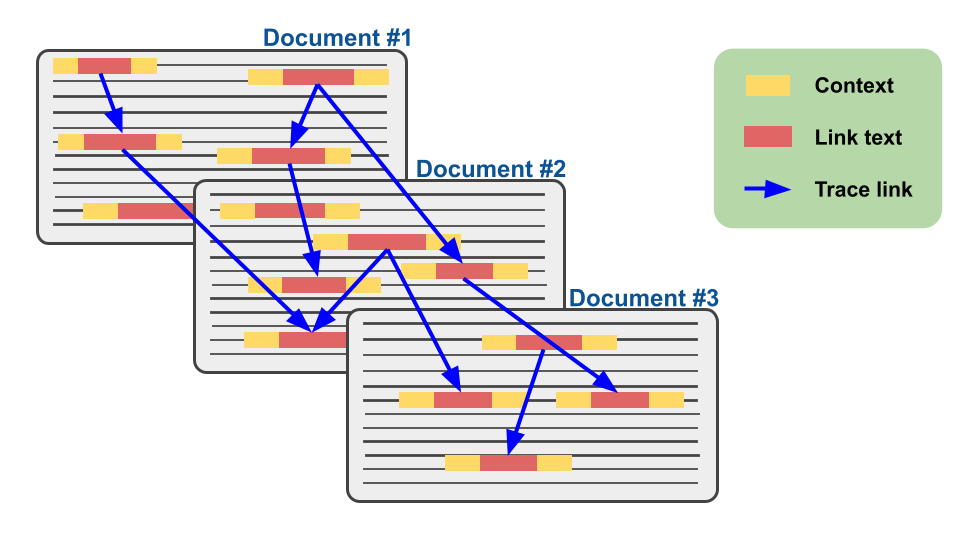
\includegraphics[width=0.85\textwidth]{use_graph}
  \caption{Random walk trace of locations visited by the policy network by querying the radix tree. These form a graph representing relevant entity links, which can be later used for prediction on a downstream task.}
\end{figure*}

During evaluation, we measure how well the agent performed. Many loss functions are possible depending on the task in question, from a simple string distance metric over a masked code fragment, to a more complex property (e.g. the presence or absence of an error, or some internal state of the REPL) which must be satisfied by interacting with the runtime environment. Many program analysis and repair tasks are amenable to the setup described, including defect, duplicate or vulnerability detection and correction.

\section{Method}

We fetch a dataset of random repositories on GitHub containing a mixture of filetypes representing both source code and natural language artifacts. Each project is indexed using a variable height radix tree, producing a multimap of prefix strings to a set of artifact, offset $(A, O)$ pairs in linear time.

 We initialize the policy network using a pretrained language model. Starting at the site of the prediction task and conditioning on the context, the policy network draws K queries from its latent state. Querying the radix tree produces a set of matching locations within the project, and the process is repeated at each location using either direct BFS traversal, or expanding a subset of most promising locations via finite-horizon MCTS.

The rollout traces form a graph of related locations inside the project and their corresponding context embeddings, which become the GNN node features. Once the rollout ends, we run message passing on the resulting GNN for a fixed numbers of steps, then decode the graph embedding. Both the decoder, GNN weights, and policy network are trained end-to-end on the downstream task, e.g. code completion, defect detection or correction.

\section{Experiments}

In this work, we attempt to understand the relationship between entities in a software project. Our research seeks to answer the following questions:

\begin{enumerate}
  \item Which kinds of artifacts in a software project are visited most often?
  \item To what degree can we claim the agent has learned to:\begin{enumerate}
  \item Locate contextually relevant artifacts within a software project?
  \item Comprehend the semantic content of the artifacts traversed?
  \item Apply the knowledge gathered to perform the assigned task?
  \end{enumerate}
\end{enumerate}

In our first experiment, we attempt to understand which queries the agent is performing when solving a programming task. Does it search for certain keywords in the context? Are those keywords relevant to the task?

In our second experiment, we try to measure the information gain from various filetypes through ablation. For trajectories containing filetypes such as Markdown or Java, what information gain do these resources provide and which filetypes are are the most salient for the prediction task?

In our third experiment, we compare prediction accuracy a variety of hyperparameters, such as search horizon depth, action space, and parameter sharing across query, GNN and decoder networks. Should we constrain the action space (e.g. by only considering query tokens from the surrounding context) for more efficient trajectory sampling, or allow arbitrary queries?

If our hypothesis is correct, the policy network will learn to use both natural language and source code artifacts. If so, this would provide evidence to support the broader hypothesis~\cite{guo2017semantically}, that documentation is a useful source of information. In addition to being useful for the prediction task itself, this could also provide a mechanism for knowledge graph extraction.

\section{Next steps}

Our next steps are to build a simple RL environment which allows an agent to interact with a software repository and construct a graph. We will use an in-memory filesystem to store and load project artifacts. The policy network will need to be pretrained on a corpus of projects in the same language. To model the action space, we will use the radix tree of the parent project, with transition probabilities conditioned on the local context.

For further details and to get started, please visit our GitHub page: \url{https://github.com/breandan/gym-fs}.

  \bibliography{research_proposal}
  \bibliographystyle{plain}
\end{document}